\chapter{Results}\label{results} 

\section{Introduction}
In order to understand the effectiveness of this proposal, an extensive computational study 
was carried out using our main algorithm $NetworkDesign$. Recall that $NetworkDesign$ 
involves a Construction Phase using $Greedy$, followed by a Local Search Phase with VNS 
(with three local searches, to know, $KeyTreeLocalSearch$, 
$KeyPathLocalSearch$ and $SwapKeyPathLocalSearch$) and the introduction of RVR for the reliability evaluation. The underlying probabilistic model is precisely the hostile model, 
where both links and Steiner nodes fail~\cite{103}. Given the monotonicity of this model, the application of RVR is suitable for this purpose. 

The experimental analysis was carried out in a laptop Pentium Core I5, 8GB. We selected 
$p_{min}=0.8$ in all the instances under study and $k=5$ for $Greedy$. 
The parameter $k$ was selected using preliminary tests under random graphs generated using 
our algorithm for the construction of test-graphs, looking for different values of $k$. The value $k=5$ showed acceptable results for those preliminary tests. Since this thesis proposes a  reliability-centric design, it makes no sense to establish a threshold that is lower than 
80\%. The elementary reliabilities for both Steiner nodes and links are close to the unit. In fact, we are focused on the design of highly-reliable networks.

\section{Description of the Test-Set}
After a literature review, a possibility is to build a test-set for the computational analysis using random graphs. We considered a random graph generation for the different algorithms 
involved in the solution, and for preliminary tests in the main algorithm $NetworkDesign$.  

In order to highlight the effectiveness of our proposal, we finally considered well-known instances from the Travelling Salesman Problem (TSP), extracted from the TSPLIB~\cite{24}. 
To the best of our knowledge, there are no benchmarks available for our particular problem. Therefore, we decided to adapt the instances from a well-known library with full accessibility. 

Some instances from TSPLIB were selected, and then they were modified to get complete graphs, with the corresponding euclidean costs on the links. Specifically, we selected the following instances under study: att48, berlin52, brazil58, ch150, d198, eil51, gr137, gr202, kroA100, kroA150, kroB100, kroB150, kroB200, lin105, pr152, rat195, st70,
tsp225, u159, rd100 and rd400. Observe that the suffix is the number of nodes in the corresponding instance (e.g., kroA100 has 100 nodes). 
The first column from Table~\ref{set} contains the name of the instance. The following columns, from the left to the right, contain respectively:
\begin{itemize}
\item \% $T$: the percentage of terminal nodes in the graph. We considered 
20\%, 35\% y 50\% for our test-set. Then, we have 3 classes of instances for each TSP instance. 
\item \% $Rel$: the elementary reliabilities for Steiner nodes and links, respectively.
\item \% $Req$: this is the percentage of pairs (terminal nodes) that should meet a connectivity requirements $r_{i,j}\in \{2,3,4\}$, respectively. 
\item $Iter\_ND$: iterations considered in $NetworkDesign$, according to \%$T$.
\item $Iter\_RVR$: iterations considered in $RVR$ method.
\item \#: number of generated instances.
\end{itemize}

The constraint imposed by the reliability threshold is carried out in a subset of test-cases, and the corresponding results are detailed in Section~\ref{results:2}. The abbreviation \emph{NA} (for non-applicable) appears for those 
instances were the reliability threshold is not performed. On the other hand, our $Greedy$ construction and the application of $VNS$ takes place over the whole test-set. 

If the name includes (E), this means that the instance is a variation of the corresponding instance, with different connectivity requirements. The number of iterations for 
$NetworkDesign$ is established in $Iter\_ND=100$ for those instances with relative small CPU times (minutes), and $Iter\_ND \in \{20,50\}$ for instances with more demanding CPU times. 
The number of iterations for the RVR method is $Iter\_RVR = 10^4$, selected again using preliminary tests.  

\begin{table}[H]
\caption{Test-Set} % title of Table
\centering  % used for centering table
\begin{tabular}{|c|c|c|c|c|c|c|c|} % centered columns 
\hline	$Problem$   &	\% $T$ & \%$Rel$& \% $Req$ & $Iter\_ND$ & $Iter\_RVR$ & \# \\
\hline	att48	&	20-35-50	&	99-95	&	100-0-0	&	100-100-100	&	$10^4$	&	3	\\
\hline	berlin52	&	20-35-50	&	99-95	&	100-0-0	&	100-100-100	&	$10^4$	&	3	\\
\hline	brazil58	&	20-35-50	&	99-95	&	100-0-0	&	100-100-100	&	$10^4$	&	3	\\
\hline	ch150	&	20-35-50	&	99-95	&	100-0-0	&	100-100-100	&	$10^4$	&	3	\\
\hline	d198	&	20-35-50	&	99-95	&	100-0-0	&	20-20-20	&	NA	&	3	\\
\hline	eil51	&	20-35-50	&	99-95	&	100-0-0	&	100-100-100	&	$10^4$	&	3	\\
\hline	gr137	&	20-35-50	&	99-95	&	100-0-0	&	100-20-20	&	NA	&	3	\\
\hline	gr202	&	20-35-50	&	99-95	&	100-0-0	&	100-100-100	&	$10^4$	&	3	\\
\hline	kroA100	&	20-35-50	&	99-95	&	100-0-0	&	100-100-100	&	NA	&	3	\\
\hline	kroA150	&	20-35-50	&	99-95	&	100-0-0	&	100-20-20	&	NA	&	3	\\
\hline	kroB100	&	20-35-50	&	99-95	&	100-0-0	&	100-100-100	&	NA	&	3	\\
\hline	kroB150	&	20-35-50	&	99-95	&	100-0-0	&	100-20-20	&	NA	&	3	\\
\hline	kroB200	&	20-35-50	&	99-95	&	100-0-0	&	20-20-20	&	NA	&	3	\\
\hline	lin105	&	20-35-50	&	99-95	&	100-0-0	&	100-100-100	&	NA	&	3	\\
\hline	pr152	&	20-35-50	&	99-95	&	100-0-0	&	20-20-20	&	NA	&	3	\\
\hline	rat195	&	20-35-50	&	99-95	&	100-0-0	&	20-20-20	&	NA	&	3	\\
\hline	st70	&	20-35-50	&	99-95	&	100-0-0	&	100-100-100	&	$10^4$	&	3	\\
\hline	tsp225	&	20-35-50	&	99-95	&	100-0-0	&	50-50-50	&	$10^4$	&	3	\\
\hline	u159	&	20-35-50	&	99-95	&	100-0-0	&	20-20-20	&	NA	&	3	\\
\hline	rd100	&	20-35-50	&	99-95	&	100-0-0	&	100-100-100	&	NA	&	3	\\
\hline	rd400	&	20-35-50	&	99-95	&	100-0-0	&	50-50-50	&	$10^4$	&	3	\\
\hline	berlin52(E)	&	20	&	99-90	&	65-25-10	&	100	&	$10^4$	&	1	\\
\hline	eil51(E)	&	20	&	99-90	&	65-25-10	&	100	&	$10^4$	&	1	\\
\hline	att48(E)	&	35	&	99-90	&	65-25-10	&	100	&	$10^4$	&	1	\\
\hline	st70(E)	&	35	&	99-90	&	65-25-10	&	100	&	$10^4$	&	1	\\
\hline	brazil58(E)	&	50	&	99-90	&	65-25-10	&	100	&	$10^4$	&	1	\\
\hline	eil51(E)	&	50	&	99-90	&	65-25-10	&	100	&	$10^4$	&	1	\\
\hline	kroB100(E)	&	20	&	99-90	&	65-25-10	&	100	&	$10^4$	&	1	\\
\hline	lin105(E)	&	20	&	99-90	&	65-25-10	&	100	&	NA	&	1	\\
\hline	kroA100(E)	&	35	&	99-90	&	65-25-10	&	20	&	$10^4$	&	1	\\
\hline	rd100(E)	&	35	&	99-90	&	65-25-10	&	20	&	NA	&	1	\\
\hline
\end{tabular}
\label{set} % is used to refer this table in the text
\end{table}

A second test-set is considered in order to answer strategic questions that represent the main 
goals of this thesis: the sensibility of the solution to perturbations in the elementary reliabilities. 
Different values for the elementary reliabilities for both Steiner nodes and links were used. 
Specifically, the nine combinations for $p_{v},p_{e} \in \{0.99, 0.97,0.95\}$ were introduced in 
different instances, being $p_v$ and $p_e$ the elementary reliabilities for Steiner nodes and 
links $e=(i,j)$ respectively. The details of the second test-set are presented in Table~\ref{set2}.  

\begin{table}[H]
\caption{Test-Set (2)} % title of Table
\centering  % used for centering table
\begin{tabular}{|c|c|c|c|c|c|c|} % centered columns 
\hline	$Problem$   &	\% $T$ & \% $Req$ & $Iter\_ND$ & $Iter\_RVR$ & \# \\
\hline	att48 &	20-35-50			&   100-0-0	&	100	&	$10^4$	&	3	\\
\hline	att48(E)	&	20	        &   0-100-0	&	100	&	$10^4$	&	1	\\
\hline	att48(E)	&	20	         &	0-0-100	&	100	&	$10^4$	&	1	\\
\hline	att48(E)	&	35       	 &	65-25-10	&100	&	$10^4$	&	1	\\
\hline	berlin52	&	20-35-50	 &	100-0-0	&	100&	$10^4$	&	3	\\
\hline	berlin52(E)	&	20	         &	65-25-10&   100	&	$10^4$	&	1	\\
\hline	brazil58	&	20-35-50	 &	100-0-0	&	100	&	$10^4$	&	3	\\
\hline	brazil58(E)	&	50	         &	65-25-10	&100	&	$10^4$	&	1	\\
\hline	eil51   	&	20-35-50	 &	100-0-0	&	100	&	$10^4$	&	3	\\
\hline	eil51(E)	&	20	         &	65-25-10	&	100	&	$10^4$	&	1	\\
\hline	eil51(E)	&	50	         &	65-25-10	&	100	&	$10^4$	&	1	\\
\hline	kroA100  	&	35	         &	100-0-0	&	100	&	$10^4$	&	1	\\
\hline	kroA100(E)  &	35	         &	65-25-10	&100	&	$10^4$	&	1	\\
\hline	kroB100	    &	20	         &	100-0-0	&	100	&	$10^4$	&	1	\\
\hline	kroB100(E)	&	20	         &	65-20-10	&100	&	$10^4$	&	1	\\
\hline	ch150    	&	20-35-50	 &	100-0-0	&	100	&	$10^4$	&	3	\\
\hline	gr202	    &	20-35-50	 &	100-0-0	&	100	&	$10^4$	&	3	\\
\hline	tsp225	    &	20-35-50	 &	100-0-0	&	100	&	$10^4$	&	3	\\
\hline	rd400	    &	20-35-50	 &	100-0-0	&	100	&	$10^4$	&	3	\\
\hline
\end{tabular}
\label{set2} % is used to refer this table in the text
\end{table}

For instance, in the first row we can see that we generate 3 instances for att48 with respective 
percentage of terminal nodes 20-35-50, where the connectivity requirements are $r_{ij}=2$ (100-0-0). 
For each instance of att48, one-hundred feasible solutions were found, using $10^4$ 
iterations of the RVR method with the nine possible scenarios of elementary reliabilities: 
$99-99, 99-97, 99-95, 97-99, 97-97, 97-95, 95-99, 95-97, 95-95$.\\
 
It is worth to mention that thousands of hours of CPU times were required for this thesis 
in order to accomplish this number of generated instances, considering the number of iterations involved in the search of locally optimum solutions during the VND, and the corresponding reliability evaluation. 
Section~\ref{results:2} reports the numerical results. As a consequence, the answers to the strategic 
questions of this thesis are provided in Section~\ref{answers}. 


\section{Numerical Results} \label{results:2}
Table~\ref{res} shows the results for each TSP instance under study. The first column contains the name of the instance. Column 2 shows the percentage of terminal nodes, and the remaining columns present, in order:
\begin{itemize}
\item \%$IG$: percentage of improvement of $Greedy$ in relation to the original cost of the instance.
\item \%$IVNS$: percentage of improvement of $VNS$, in relation with the output of our $Greedy$ construction.
\item $CPU$: average CPU-time per iteration of $NetworkDesign$. %%%CUIDADO CAMBIAR TP-I POR CPU
\item $\overline{R}$: average for the reliability estimation. 
\item $\overline{Var}$: average for the estimated variance.
\end{itemize} 

\begin{center}
\begin{longtable}{|l|l|l|l|l|l|l|}
\caption{\textbf{Numerical Results}}\label{res}\\ % is used to refer this table in the text
%\centering  % used for centering table

\hline \multicolumn{1}{|c|}{$Problem$} & \multicolumn{1}{c|}{\% $T$} & 
\multicolumn{1}{c|}{\%$IG$} & \multicolumn{1}{c|}{\% $IVNS$}  &
\multicolumn{1}{c|}{\textbf{$CPU$ (s)}} & \multicolumn{1}{c|}{$\overline{R}$}  &
\multicolumn{1}{c|}{$\overline{Var}$} \\ \hline 
\endfirsthead


\multicolumn{7}{c}%
{{\bfseries \tablename\ \thetable{}-- Numerical Results (cont.)}} \\
\hline \multicolumn{1}{|c|}{$Problem$} & \multicolumn{1}{c|}{\% $T$} & 
\multicolumn{1}{c|}{\%$IG$} & \multicolumn{1}{c|}{\% $IVNS$}  &
\multicolumn{1}{c|}{\textbf{$CPU$ (s)}} & \multicolumn{1}{c|}{$\overline{R}$}  &
\multicolumn{1}{c|}{$\overline{Var}$} \\ \hline 
\endhead

\multicolumn{7}{c}%
{{\bfseries \tablename\ \thetable{} -- Numerical Results (cont.)}} \\
\hline \multicolumn{1}{|c|}{$Problem$} & \multicolumn{1}{c|}{\% $T$} & 
\multicolumn{1}{c|}{\%$IG$} & \multicolumn{1}{c|}{\% $IVNS$}  &
\multicolumn{1}{c|}{\textbf{$CPU$ (s)}} & \multicolumn{1}{c|}{$\overline{R}$}  &
\multicolumn{1}{c|}{$\overline{Var}$} \\ \hline 
\endhead

%\hline \multicolumn{7}{|r|}{{Continued on next page}} \\ \hline
\endfoot

\hline \hline
\endlastfoot


%\hline	$Problem$   &	\% $T$ & \%$IG$& \% $IVNS$ & $CPU$ & $\overline{R}$ & $\overline{Var}$ \\
\hline	att48	&	20	&	99.27	&	34.61	&	11.466	&	96.7	&	7.608E-07	\\
\hline	att48	&	35	&	98.6	&	36.83	&	29.769	&	94.3	&	3.448E-06	\\
\hline	att48	&	50	&	98.22	&	37.1	&	65.904	&	92.7	&	5.322E-06	\\
\hline	berlin52	&	20	&	98.98	&	30.55	&	30.605	&	93.7	&	3.294E-06	\\
\hline	berlin52	&	35	&	99.06	&	33.93	&	33.433	&	93.8	&	3.19E-06	\\
\hline	berlin52	&	50	&	98.02	&	33.48	&	106.945	&	90.7	&	6.487E-06	\\
\hline	brazil58	&	20	&	98.92	&	31.96	&	62.377	&	88.5	&	6.722E-06	\\
\hline	brazil58	&	35	&	99.25	&	39.45	&	68.891	&	86	&	8.347E-06	\\
\hline	brazil58	&	50	&	98.75	&	35.26	&	103.553	&	91	&	7.093E-06	\\
\hline	ch150	&	20	&	99.76	&	37.51	&	222.552	&	85.59	&	1.029E-05	\\
\hline	ch150	&	35	&	99.72	&	36.65	&	546.652	&	88.03	&	9.033E-05	\\
\hline	ch150	&	50	&	99.69	&	34.42	&	1203.054	&	88.8	&	8.974E-05	\\
\hline	d198	&	20	&	99.9	&	32.22	&	320.142	&	NA	&	NA	\\
\hline	d198	&	35	&	99.86	&	34.12	&	2086.376	&	NA	&	NA	\\
\hline	d198	&	50	&	99.81	&	33.39	&	5548.639	&	NA	&	NA	\\
\hline	eil51	&	20	&	99.34	&	38.79	&	14.87	&	96	&	1.183E-06	\\
\hline	eil51	&	35	&	98.54	&	36.11	&	39.017	&	94.2	&	3.736E-06	\\
\hline	eil51	&	50	&	98.56	&	37.32	&	44.798	&	93.7	&	4.284E-06	\\
\hline	gr137	&	20	&	99.79	&	36.31	&	137.496	&	NA	&	NA	\\
\hline	gr137	&	35	&	99.71	&	34.18	&	404.061	&	NA	&	NA	\\
\hline	gr137	&	50	&	99.68	&	34.61	&	976.369	&	NA	&	NA	\\
\hline	gr202	&	20	&	99.89	&	32.43	&	528.162	&	82.31	&	1.224E-05	\\
\hline	gr202	&	35	&	99.75	&	34.56	&	3511.698	&	84.14	&	1.11E-05	\\
\hline	gr202	&	50	&	99.74	&	33.36	&	9505.629	&	83.03	&	1.279E-05	\\
\hline	kroA100	&	20	&	99.61	&	36.77	&	44.225	&	NA	&	NA	\\
\hline	kroA100	&	35	&	99.53	&	38.23	&	101.498	&	88.97	&	8.525E-05	\\
\hline	kroA100	&	50	&	99.45	&	35.89	&	280.833	&	NA	&	NA	\\
\hline	kroA150	&	20	&	99.83	&	36.7	&	102.712	&	NA	&	NA	\\
\hline	kroA150	&	35	&	99.75	&	36.3	&	412.97	&	NA	&	NA	\\
\hline	kroA150	&	50	&	99.7	&	32.32	&	2035.062	&	NA	&	NA	\\
\hline	kroB100	&	20	&	99.68	&	38.71	&	17.301	&	90.14	&	6.251E-05	\\
\hline	kroB100	&	35	&	99.59	&	36.32	&	53.74	&	NA	&	NA	\\
\hline	kroB100	&	50	&	99.49	&	34.98	&	191.722	&	NA	&	NA	\\
\hline	kroB150	&	20	&	99.84	&	37.49	&	112.099	&	NA	&	NA	\\
\hline	kroB150	&	35	&	99.77	&	36.05	&	665.676	&	NA	&	NA	\\
\hline	kroB150	&	50	&	99.73	&	34.53	&	1327.528	&	NA	&	NA	\\
\hline	kroB200	&	20	&	99.89	&	36.14	&	279.156	&	NA	&	NA	\\
\hline	kroB200	&	35	&	99.84	&	35.06	&	2234.738	&	NA	&	NA	\\
\hline	kroB200	&	50	&	99.8	&	33.82	&	7448.424	&	NA	&	NA	\\
\hline	lin105	&	20	&	99.74	&	35.89	&	9.439	&	NA	&	NA	\\
\hline	lin105	&	35	&	99.61	&	37.04	&	86.855	&	NA	&	NA	\\
\hline	lin105	&	50	&	99.5	&	36.4	&	245.246	&	NA	&	NA	\\
\hline	pr152	&	20	&	99.79	&	37.14	&	281.166	&	NA	&	NA	\\
\hline	pr152	&	35	&	99.77	&	36.86	&	808.477	&	NA	&	NA	\\
\hline	pr152	&	50	&	99.74	&	36.88	&	1673.465	&	NA	&	NA	\\
\hline	rat195	&	20	&	99.88	&	37.31	&	280.948	&	NA	&	NA	\\
\hline	rat195	&	35	&	99.82	&	34.7	&	1925.985	&	NA	&	NA	\\
\hline	rat195	&	50	&	99.8	&	34.99	&	4599.873	&	NA	&	NA	\\
\hline	st70	&	20	&	99.44	&	39.84	&	39.852	&	91.9	&	4.072E-06	\\
\hline	st70	&	35	&	99.3	&	39.56	&	63.65	&	90.6	&	5.743E-06	\\
\hline	st70	&	50	&	99.16	&	36.37	&	128.195	&	91.3	&	7.027E-06	\\
\hline	tsp225	&	20	&	99.88	&	34.98	&	1658.773	&	84.75	&	1.141E-05	\\
\hline	tsp225	&	35	&	99.85	&	34.65	&	4684.367	&	84.64	&	1.249E-05	\\
\hline	tsp225	&	50	&	99.82	&	33.26	&	12088.726	&	87.19	&	1.092E-05	\\
\hline	u159	&	20	&	99.81	&	35.84	&	333.263	&	NA	&	NA	\\
\hline	u159	&	35	&	99.76	&	36.14	&	864.992	&	NA	&	NA	\\
\hline	u159	&	50	&	99.75	&	35.61	&	1278.13	&	NA	&	NA	\\
\hline	rd100	&	20	&	99.68	&	37.15	&	22.421	&	NA	&	NA	\\
\hline	rd100	&	35	&	99.5	&	34.54	&	126.822	&	NA	&	NA	\\
\hline	rd100	&	50	&	99.42	&	36.13	&	245.827	&	NA	&	NA	\\
\hline	rd400	&	20	&	99.94	&	35.84	&	5000.214	&	80.94	&	14.22E-05	\\
\hline	rd400	&	35	&	99.94	&	33.54	&	9000.103	&	85.37	&	11.89E-05	\\
\hline	rd400	&	50	&	99.93	&	33.16	&	19000.70	&	86.43	&	11.51E-05	\\
\hline	berlin52(E)	&	20	&	98.45	&	25.25	&	34.209	&	99.3	&	4.848E-07	\\
\hline	eil51(E)	&	20	&	98.47	&	28.45	&	29.623	&	99.6	&	2.707E-07	\\
\hline	att48(E)	&	35	&	97.45	&	31.74	&	62.967	&	99.4	&	4.93E-07	\\
\hline	st70(E)	&	35	&	98.52	&	31.87	&	135.508	&	99.3	&	6.549E-07	\\
\hline	brazil58(E)	&	50	&	97.48	&	31.84	&	172.636	&	99.4	&	4.825E-07	\\
\hline	eil51(E)	&	50	&	97.26	&	32.67	&	74.473	&	99.1	&	7.942E-07	\\
\hline	kroB100(E)	&	20	&	99.37	&	30.25	&	39.255	&	99.87	&	1.219E-06	\\
\hline	lin105(E)	&	20	&	99.33	&	31.95	&	64.409	&	NA	&	NA	\\
\hline	kroA100(E)	&	35	&	98.99	&	35.88	&	225.505	&	99.81	&	1.828E-06	\\
\hline	rd100(E)	&	35	&	99.15	&	35.3	&	130.008	&	NA	&	NA	\\
\hline Average     & NA    &   99.39   &  35.03   &    1026.003 &  91.38 & 2.33E-05 \\
\hline
\end{longtable}
\end{center}
The improvement of $VNS$ over the constructed solution in Greedy, $IVNS$, is bounded between 
25,25\% and 39,84\%, according to the instance an its characteristics on the test-set.\\

The minimum threshold $p_{min}=0.8$ is widely exceeded in all the instances where the 
average reliability $\overline{R}$ was estimated. For those instances in which the 
elementary reliabilities were established in 99\%-95\% respectively for nodes and links, 
the range of reliabilities is bounded between 82,31\%-96,7\%, while a range of 
99,1\% y 99,87\% is observed with elementary reliabilities 99\%-90\%.\\


The estimated variance is reduced in average in all the instances under study. This suggests that 
the RVR method is accurate, even under reliability failures of $q=10^{-2}$ for both Steiner nodes and links. This fact is discussed in Section~\ref{answers}. In general, the CPU times are non-prohibitive and in general are acceptable under all the test-set. In Section~\ref{topologies}, illustrative examples of resulting networks returned by $NetworkDesign$ are presented to explain the instances defined in the previous tables.

\subsection{Resulting Topologies}\label{topologies}
\subsection*{Brazil58}
Consider Brazil58 instance with at least \%20 of terminal nodes, elementary reliability in 
Steiner nodes \%99, link-reliabilities \%95 and \%100 of 2 node-disjoint paths between each pair 
of terminal nodes as the connectivity requirement. Figures~\ref{br1} and \ref{br2} show correspondingly 
the ground graph $G_B$ and the output of $NetworkDesign$. The resulting cost is 25106, and the 
reliability is 0.917399. In Figure~\ref{br1}, the ground graph is illustrated, and the the excluded nodes and links are colored in grey. In Figure~\ref{br2}, red nodes are the terminals that do not fail, and 
Steiner nodes are represented in orange. To simplify, all the links have unit-cost.  


\begin{figure}
\begin{center}
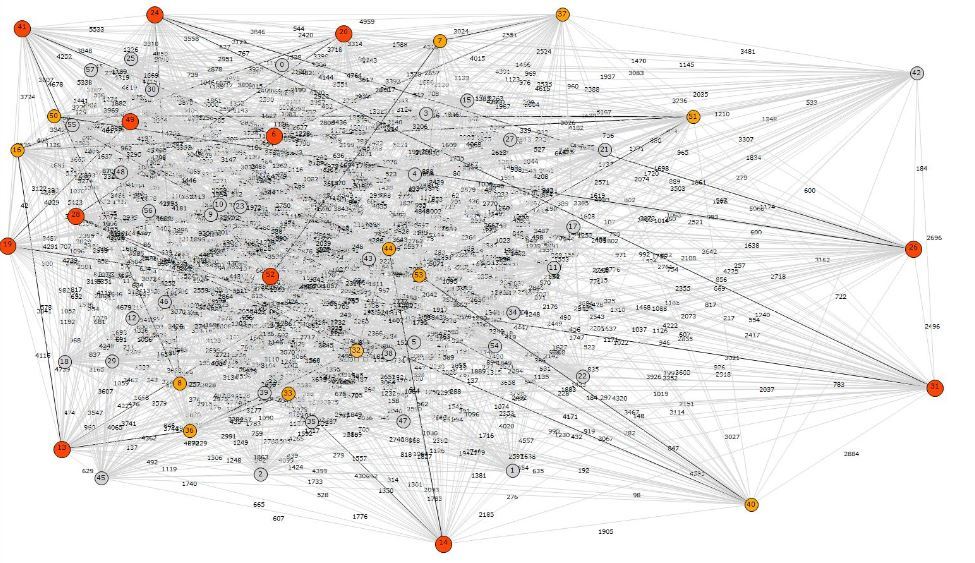
\includegraphics[scale=0.55]{1.jpg}
\caption{Brazil58: ground graph $G_B$.}\label{br1}
\end{center} 
\end{figure}

\begin{figure}
\begin{center}
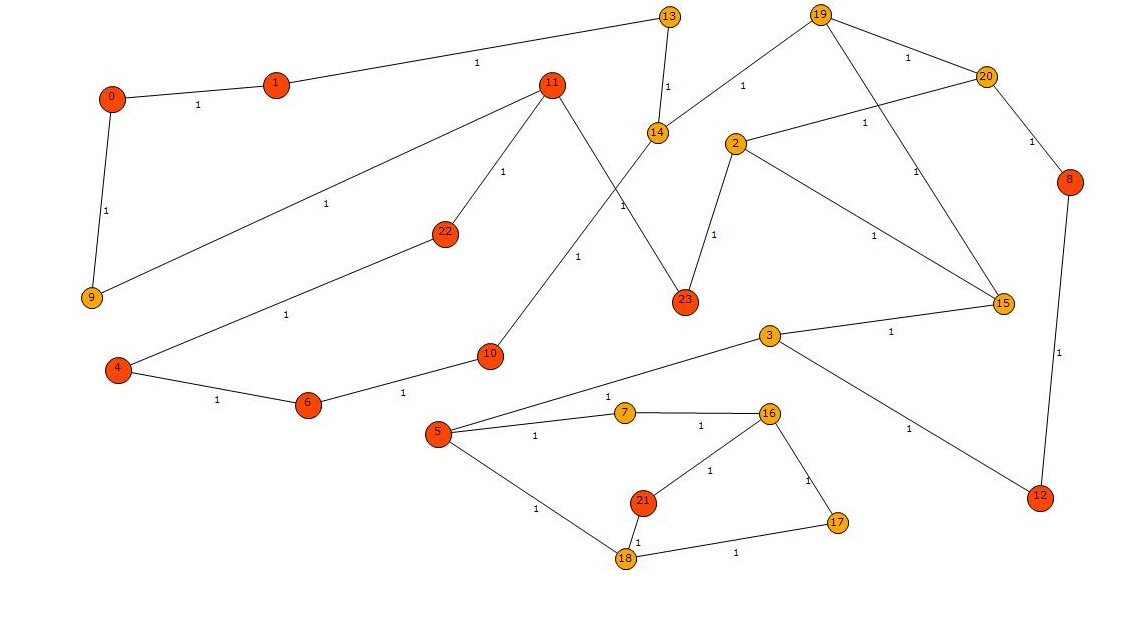
\includegraphics[scale=0.5]{2.jpg}
\caption{Brazil58: resulting topology.}\label{br2}
\end{center} 
\end{figure}


\subsection*{Berlin52}
Consider Berlin52 instance under identical conditions, with at least \%20 of terminal nodes, elementary reliability in Steiner nodes \%99, link-reliabilities \%95 and \%100 of 2 node-disjoint paths between each pair 
of terminal nodes as the connectivity requirement. Figures~\ref{be1} and \ref{be2} show correspondingly 
the ground graph $G_B$ and the output of $NetworkDesign$. The resulting cost is 4534.109370, and the 
reliability is 0.844772. In Figure~\ref{be1}, the ground graph is illustrated, and the excluded nodes and links are colored in grey. In Figure~\ref{be2}, red nodes are the terminals that do not fail, and 
Steiner nodes are represented in orange. To simplify, all the links have unit-cost.  

\begin{figure}[H]
\begin{center}
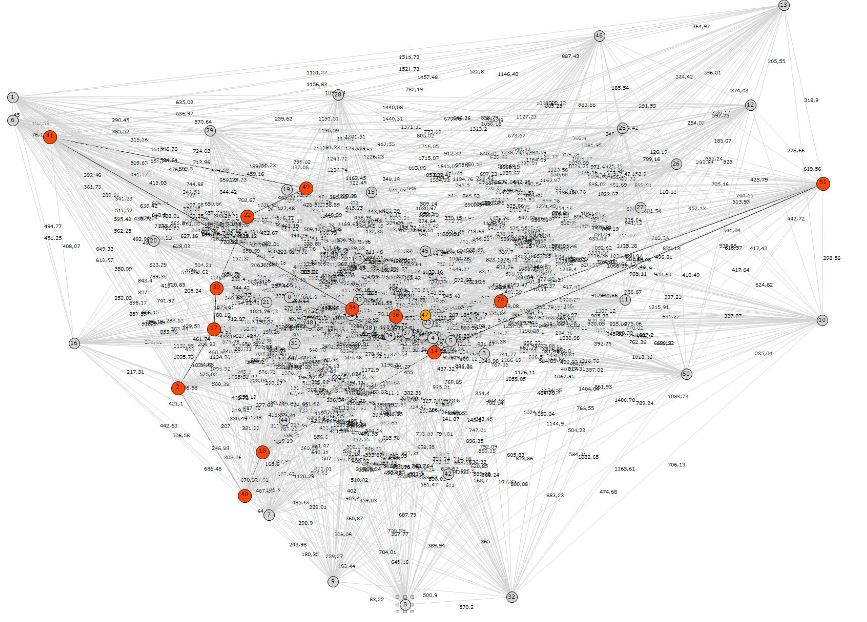
\includegraphics[scale=0.6]{3.jpg}
\caption{Berlin52: ground graph $G_B$.}\label{be1}
\end{center} 
\end{figure}

\begin{figure}[H]
\begin{center}
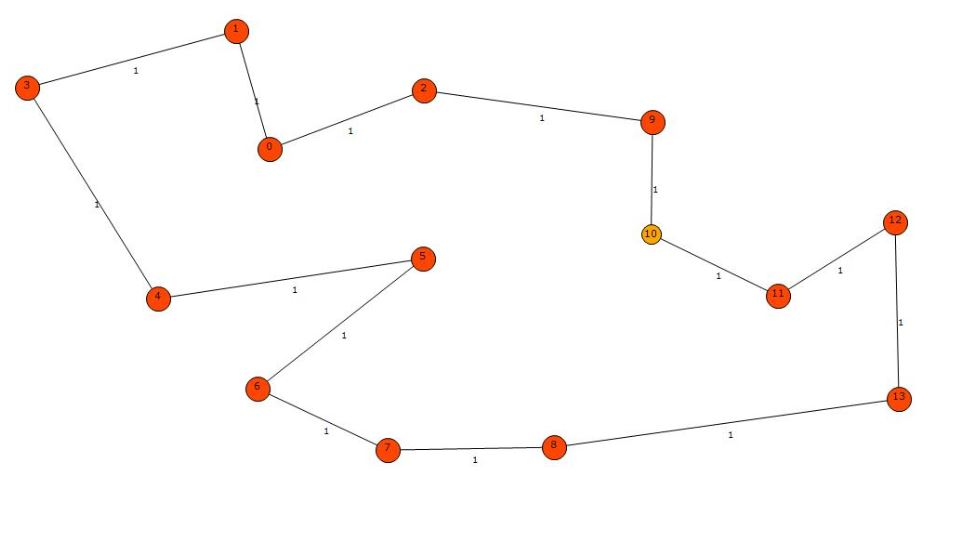
\includegraphics[scale=0.55]{4.jpg}
\caption{Berlin52: resulting topology.}\label{be2}
\end{center} 
\end{figure}

\clearpage
\section{Key Questions}\label{answers}
Our particular interest is to answer the following questions that relate the network optimization and 
reliability evaluation stages that were addressed throughout this work. 
\begin{question}
How many feasible networks there exists given the full probabilistic model $(p_{min},P_E,P_{V-T})$? 
\end{question}

We will restrict our attention to the number of feasible networks that we \emph{can find}, for specific 
values in the probabilistic model. Nevertheless, this information gives us an insight of the level of feasibility 
provided by our main algorithm $NetworkDesign$, which serves as a guide, and to offer partial answers. 
Consider $p_{min}=0.98$ and different percentage of solutions that survived for the pair 
of identical elementary reliabilities in Steiner nodes and links \%99-\%99. 
The respective percentages under different instances is presented in Table~\ref{answer1}. 
We can appreciate that, in general, the number of solutions that meet the reliability threshold is high. 
Indeed, it is 100\% of the returned solutions in most instances. 

\begin{table}
\caption{Percentage of feasible solutions such that $R \geq 0.98$} % title of Table
\centering  % used for centering table
\begin{tabular}{|c|c|c|} % centered columns 
\hline	Rel \%99-\%99   &	\% Feasible solutions with $R \geq 0.98$ \\
\hline	att48 T20	&	100	\\
\hline	att48 T35	&	100	\\
\hline	att48 T50	&	100	\\
\hline	eil51 T20	&	100	\\
\hline	eil51 T35	&	100	\\
\hline	eil51 T50	&	100	\\
\hline	berlin52 T20	&	100	\\
\hline	berlin52 T35	&	100	\\
\hline	berlin52 T50	&	100	\\
\hline	brazil58 T20	&	99	\\
\hline	brazil58 T35	&	97	\\
\hline	brazil58 T50	&	100	\\
\hline	ch150 T20	&	100	\\
\hline	ch150 T35	&	100	\\
\hline	ch150 T50	&	100	\\
\hline	gr202 T20	&	99	\\
\hline	gr202 T35	&	100	\\
\hline	gr202 T50	&	100	\\
\hline	tsp225 T20	&	100	\\
\hline	tsp225 T35	&	100	\\
\hline	tsp225 T50	&	100	\\
\hline	rd400 T20	&	100	\\
\hline	rd400 T35	&	100	\\
\hline	rd400 T50	&	100	\\
\hline
\end{tabular}
\label{answer1} % is used to refer this table in the text
\end{table}

\begin{question}
What is the sensibility of the model with respect to the elementary reliabilities? 
For instance, for any given threshold ($p_{min}=0.98$), what happens if we fix 
$p_v=0.99$ but we pick different values for the elementary link reliabilities 
$p_e \in \{0.99,0.97,0.95\}$? How many feasible networks survive? Analogously, if we 
fix $p_e=0.99$ and $p_v \in \{0.99, 0.97, 0.95\}$. 
\end{question}

Consider the threshold $p_{min}=0.98$. Tables~\ref{answer2a} and~\ref{answer2b} present the percentage of feasible solutions under different scenarios.

On one hand, if we fix the node-reliability and reduce the elementary link-reliabilities, a notorious reduction in 
the number of feasible solutions is observed, even reaching $0$ in almost-all the instances under study 
when the link-reliabilities are \%95. It is worth to note that the feasibility is also 0 specially 
in large networks when the link reliabilities are \%97. This pattern for the results is reasonable, since the number of links is also increased when the size of the network is larger.

On the other hand, if we fix the link-reliabilities and reduce the node-reliabilities, the 
reduction in the reliability is less important than in the previous setting, in terms of 
the percentage of feasible solutions. We can appreciate that if the number of terminal-nodes is decreased, 
the corresponding reduction in the percentage of feasible solutions that exceed the threshold $p_{min}$ is 
not as steep as in the previous case. This is coherent, since larger networks have more perfect terminal nodes 
(recall that Steiner nodes are optional). Nevertheless, the global effect of network expansion is a corresponding reduction in the percentage of solutions that exceed the reliability threshold, since the number of Steiner nodes is increased. This reduction is not as steep as in the previous case. 

\begin{table}
\caption{Solutions such that $R \geq 0.98$ ($p_v$ fixed)} % title of Table
\centering  % used for centering table
\begin{tabular}{|c|c|c|c|c|} % centered columns 
\hline	$Rel$ \%99-\%x  &	\%99-\%99 & \%99-\%97 & \%99-\%95\\
\hline	att48 T20	&	100	&	90	&	12	\\
\hline	att48 T35	&	100	&	53	&	0	\\
\hline	att48 T50	&	100	&	20	&	0	\\
\hline	berlin52 T20	&	100	&	41	&	0	\\
\hline	berlin52 T35	&	100	&	50	&	0	\\
\hline	berlin52 T50	&	100	&	1	&	0	\\
\hline	brazil58 T20	&	99	&	15	&	0	\\
\hline	brazil58 T35	&	97	&	0	&	0	\\
\hline	brazil58 T50	&	100	&	5	&	0	\\
\hline	ch150 T20	&	100	&	0	&	0	\\
\hline	ch150 T35	&	100	&	0	&	0	\\
\hline	ch150 T50	&	100	&	0	&	0	\\
\hline	gr202 T20	&	99	&	0	&	0	\\
\hline	gr202 T35	&	100	&	0	&	0	\\
\hline	gr202 T50	&	100	&	0	&	0	\\
\hline	rd400 T20	&	100	&	0	&	0	\\
\hline	rd400 T35	&	100	&	0	&	0	\\
\hline	rd400 T50	&	100	&	0	&	0	\\
\hline
\end{tabular}
\label{answer2a} % is used to refer this table in the text
\end{table}

\begin{table}
\caption{Solutions such that $R \geq 0.98$ ($p_e$ fixed)} % title of Table
\centering  % used for centering table
\begin{tabular}{|c|c|c|c|c|} % centered columns 
\hline	$Rel$ \%x-\%99  &	\%99-\%99 & \%97-\%99 & \%95-\%99\\
\hline	tt48 T20	&	100	&	100	&	99	\\
\hline	att48 T35	&	100	&	98	&	96	\\
\hline	att48 T50	&	100	&	100	&	99	\\
\hline	berlin52 T20	&	100	&	100	&	80	\\
\hline	berlin52 T35	&	100	&	99	&	93	\\
\hline	berlin52 T50	&	100	&	100	&	100	\\
\hline	brazil58 T20	&	99	&	59	&	41	\\
\hline	brazil58 T35	&	97	&	43	&	9	\\
\hline	brazil58 T50	&	100	&	99	&	81	\\
\hline	ch150 T20	&	100	&	60	&	20	\\
\hline	ch150 T35	&	100	&	98	&	76	\\
\hline	ch150 T50	&	100	&	100	&	97	\\
\hline	gr202 T20	&	99	&	80	&	30	\\
\hline	gr202 T35	&	100	&	69	&	16	\\
\hline	gr202 T50	&	100	&	100	&	76	\\
\hline	rd400 T20	&	100	&	16	&	2	\\
\hline	rd400 T35	&	100	&	98	&	80	\\
\hline	rd400 T50	&	100	&	100	&	100	\\
\hline
\end{tabular}
\label{answer2b} % is used to refer this table in the text
\end{table}

\begin{question}
How many networks survive on average, for any given probabilistic model? 
Understand the sensibility of the model with respect to the connectivity requirements 
$r_{i,j} \in \{2,3,4\}$.
\end{question}

Consider $p_{min}=0.98$. The notation \emph{$name$ $TXX$ ($Z1-Z2-Z3$)} 
means the name of the graph, $TXX$ is the percentage of terminal-nodes and $Z1-Z2-Z3$ the percentage of 
terminal nodes with connectivity requirements 2, 3 and 4 respectively. 
For example, \emph{eil51 T50 (65-25-10)} means that the instance is eil51, with 50\% of terminal nodes, 
where 65\% have connectivity requirement 2, 25\% have requirement 3 and 10\% have requirement equal to 4.

From Table~\ref{answer3}, we can appreciate that an increase in the network connectivity requirements 
necessarily imply a corresponding increase in the percentage of networks that meet the reliability 
threshold, and vice-versa. This is a nice interplay between topological network design and network 
reliability analysis: a more \emph{robust} network in a deterministic manner (node-disjoint paths) 
is translated into a most-reliable network (under probabilistic models), and vice-versa.  

\begin{table}
\caption{Solutions such that $R \geq 0.98$ (case \%99-\%97)} % title of Table
\centering  % used for centering table
\begin{tabular}{|c|c|c|} % centered columns 
\hline	Rel \%99-\%97   &	\% Feasible solutions with $R \geq 0.98$ \\
\hline	att48 T20 (100-0-0)	&	90	\\
\hline	att48 T20 (65-25-10)	&	100	\\
\hline	att48 T20 (0-100-0)	&	100	\\
\hline	att48 T20 (0-0-100)	&	100	\\
\hline	eil51 T20 (100-0-0)	&	76	\\
\hline	eil51 T20 (65-25-10)	&	100	\\
\hline	eil51 T50 (100-0-0)	&	54	\\
\hline	eil51 T50 (65-25-10)	&	100	\\
\hline	berlin52 T20 (100-0-0)	&	41	\\
\hline	berlin52 T20 (65-25-10)	&	100	\\
\hline	brazil58 T50 (100-0-0)	&	5	\\
\hline	brazil58 T50 (65-25-10)	&	100	\\
\hline	kroA100 T35 (100-0-0)	&	0	\\
\hline	kroA100 T35 (65-25-10)	&	100	\\
\hline	kroB100 T20 (100-0-0)	&	3	\\
\hline	kroB100 T20 (65-25-10)	&	100	\\
\hline
\end{tabular}
\label{answer3} % is used to refer this table in the text
\end{table}

\begin{question}
Is it better to  improve the elementary reliability of links, or the reliability of Steiner nodes, in order to meet a demanding reliability threshold? 
\end{question}

We can appreciate from Tables~\ref{answer2a} and \ref{answer2b} that an increase in the link-reliabilities 
have a better impact than a corresponding increase in node-reliabilities. 

%it is better to improve the 
%reliability of the links
%
%Del an\'alisis de los resultados en la pregunta 2 vemos que claramente tiene un mayor impacto
%sobre las soluciones \'optimas que satisfagan el umbral, el aumento de la confiabilidad en las
%aristas.
%
%
%\begin{table}[H]
%\caption{Solutions such that $R \geq 0.98$ ($p_v$ fixed)} % title of Table
%\centering  % used for centering table
%\begin{tabular}{|c|c|c|c|c|} % centered columns 
%\hline	$Rel$ \%99-\%x  &	\%99-\%99 & \%99-\%97 & \%99-\%95\\
%\hline	att48 T20	&	100	&	90	&	12	\\
%\hline	att48 T35	&	100	&	53	&	0	\\
%\hline	att48 T50	&	100	&	20	&	0	\\
%\hline	berlin52 T20	&	100	&	41	&	0	\\
%\hline	berlin52 T35	&	100	&	50	&	0	\\
%\hline	berlin52 T50	&	100	&	1	&	0	\\
%\hline	brazil58 T20	&	99	&	15	&	0	\\
%\hline	brazil58 T35	&	97	&	0	&	0	\\
%\hline	brazil58 T50	&	100	&	5	&	0	\\
%\hline	ch150 T20	&	100	&	0	&	0	\\
%\hline	ch150 T35	&	100	&	0	&	0	\\
%\hline	ch150 T50	&	100	&	0	&	0	\\
%\hline	gr202 T20	&	99	&	0	&	0	\\
%\hline	gr202 T35	&	100	&	0	&	0	\\
%\hline	gr202 T50	&	100	&	0	&	0	\\
%\hline	rd400 T20	&	100	&	0	&	0	\\
%\hline	rd400 T35	&	100	&	0	&	0	\\
%\hline	rd400 T50	&	100	&	0	&	0	\\
%\hline
%\end{tabular}
%\label{answer4a} % is used to refer this table in the text
%\end{table}
%
%\begin{table}[H]
%\caption{Solutions such that $R \geq 0.98$ ($p_e$ fixed)} % title of Table
%\centering  % used for centering table
%\begin{tabular}{|c|c|c|c|c|} % centered columns 
%\hline	$Rel$ \%x-\%99  &	\%99-\%99 & \%97-\%99 & \%95-\%99\\
%\hline	tt48 T20	&	100	&	100	&	99	\\
%\hline	att48 T35	&	100	&	98	&	96	\\
%\hline	att48 T50	&	100	&	100	&	99	\\
%\hline	berlin52 T20	&	100	&	100	&	80	\\
%\hline	berlin52 T35	&	100	&	99	&	93	\\
%\hline	berlin52 T50	&	100	&	100	&	100	\\
%\hline	brazil58 T20	&	99	&	59	&	41	\\
%\hline	brazil58 T35	&	97	&	43	&	9	\\
%\hline	brazil58 T50	&	100	&	99	&	81	\\
%\hline	ch150 T20	&	100	&	60	&	20	\\
%\hline	ch150 T35	&	100	&	98	&	76	\\
%\hline	ch150 T50	&	100	&	100	&	97	\\
%\hline	gr202 T20	&	99	&	80	&	30	\\
%\hline	gr202 T35	&	100	&	69	&	16	\\
%\hline	gr202 T50	&	100	&	100	&	76	\\
%\hline	rd400 T20	&	100	&	16	&	2	\\
%\hline	rd400 T35	&	100	&	98	&	80	\\
%\hline	rd400 T50	&	100	&	100	&	100	\\
%\hline
%\end{tabular}
%\label{answer4b} % is used to refer this table in the text
%\end{table}